\chapter{Experiment Setup ~20}

\section{Jefferson Lab CEBAF}

The PRex and CREx experiments are conducted at the Continuous Electron Beam Accelerator Facility (CEBAF) housed within Jefferson Lab. Since its inception in the early 1990s, CEBAF has been a global pioneer, forging paths in nuclear physics research.

The heart of CEBAF is its linear accelerators (linacs), specifically the North and South linacs. These linacs serve as the key elements where electrons amass energy, essential for the facility's experimental proceedings. Connecting these two linacs are the Recirculation Arcs, which are magnetic systems designed to curve the electron beam, redirecting it back into the linacs for additional energy enhancement during successive passes. An added function of the Recirculation Arcs is to facilitate the separation of electron beams of varying energy levels, post their multiple circulations through the linacs. This structural alignment and the operational interplay between the components ensure precision and efficacy in executing complex nuclear physics experiments like PRex and CRex.


% Para. 2
% \begin{itemize}
%     \item 12GeV upgrade
%     \item RF separator
%     \item RF cavities, cooled 
%     \item Beam energy and current ability
%     \item accelerated up to 5 times though both linacs, producing a nominal energy of 10.9GeV. 
%     \item 1497MhZ split into three 499MHz.
%     \item north and south linacs each can gen 1.1GeV 
%     \item East/West Arc bend the beam to accelerate again 
%     \item Hall ABC, 10.9GeV 
%     \item Hall D 12GeV
% \end{itemize}

The Jefferson Lab's CEBAF upgrade project, completed in 2014, introduced a number of significant enhancements. The modifications included the addition of five cryomodules to each Linac section, each housing 7-cell cavities capable of handling a higher RF field, courtesy of advanced surface treatments.

Each of these upgraded linacs can now facilitate an energy gain of 1.1 GeV, enabling the electron beam to achieve 2.2 GeV during each circulation. Post traversing the south linac, the electron beam can be partitioned into three distinct 499 MHz beams.

The facility's design allows for the electron beam to be accelerated up to five times through both linacs, producing a nominal energy output of 10.9 GeV. Experimental Halls A, B, and C each can receive a beam carrying energy that is one-fifth of the full 5-pass energy. Additionally, the beam directed to Hall D can be re-accelerated in the north linac, reaching energy levels as high as 12 GeV. This upgrade has elevated the capacity and flexibility of the CEBAF, further enhancing its research potential.

% Para. 3
% \begin{itemize}
%     \item PRex requires high polarized beam 
%     \item high current to be able to get enough statistics to be able to measure 
%     \item PRex experiment choose CEBAF
%     \item high current
%     \item polarize beam ability
% \end{itemize}

The PRex-II and CREx experiments aim to quantify the thickness of the neutron skin by analyzing parity-violated asymmetry. To achieve a reliable measurement with a sufficient confidence interval, a significant volume of statistical data is required. This necessity is met by the capabilities of CEBAF, which can generate a polarized electron beam with a current reaching up to $200 uA$ and a polarization level in the range of $80-90\%$. Such robust performance plays a pivotal role in enabling the execution and success of the PRex and CREx experiments.


\begin{figure}
     \centering
     \begin{subfigure}[b]{0.45\textwidth}
         \centering
         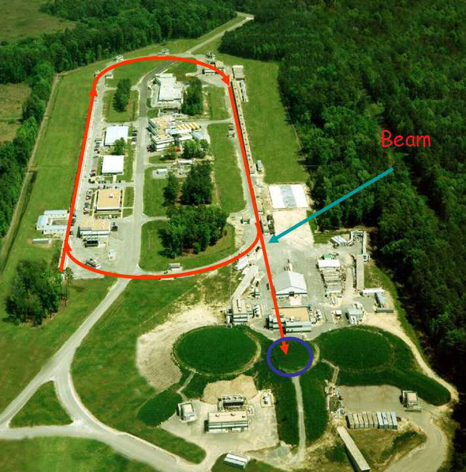
\includegraphics[width=\textwidth]{images/chap3/JLab_cebaf_photo.png}
         \caption{Photo of CEBAF}
         \label{Photo of CEBAF}
     \end{subfigure}
     \hfill
     \begin{subfigure}[b]{0.45\textwidth}
         \centering
         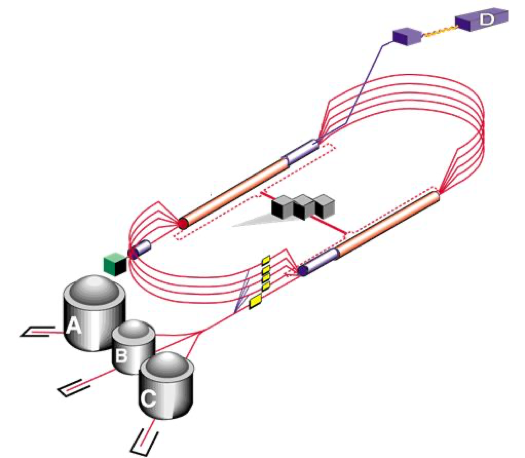
\includegraphics[width=\textwidth]{images/chap3/JLab_cebaf.png}
         \caption{JLAB CEBAF}
         \label{JLAB CEBAF}
     \end{subfigure}
\end{figure}

\section{Beam injection}
% Para. 1 & 2
% \begin{itemize}
%     \item key componet to generate polarized beam
%     \item GaAs photocathode
%     \item three different structure $30-40\%$, $50\%$, $100\%$ which is using now. Engy band plot
%     \item plot/structure of the GaAs photocathode
% \end{itemize}

The polarized electron source at Jefferson Lab comprises a specialized polarized laser system and gallium arsenide (GaAs) photocathodes. This integral apparatus permits the generation of a polarized, or spin-aligned, electron beam. This feature is indispensable for a broad range of experiments conducted at our facility, particularly those probing spin-dependent phenomena.

The GaAs photocathode is irradiated with circularly polarized laser light possessing energy exceeding the bandgap energy. This triggers the emission of electrons that exhibit specific spin polarization, a process attributable to the photoelectric effect.

\begin{figure}[!htbp]
    \centering
    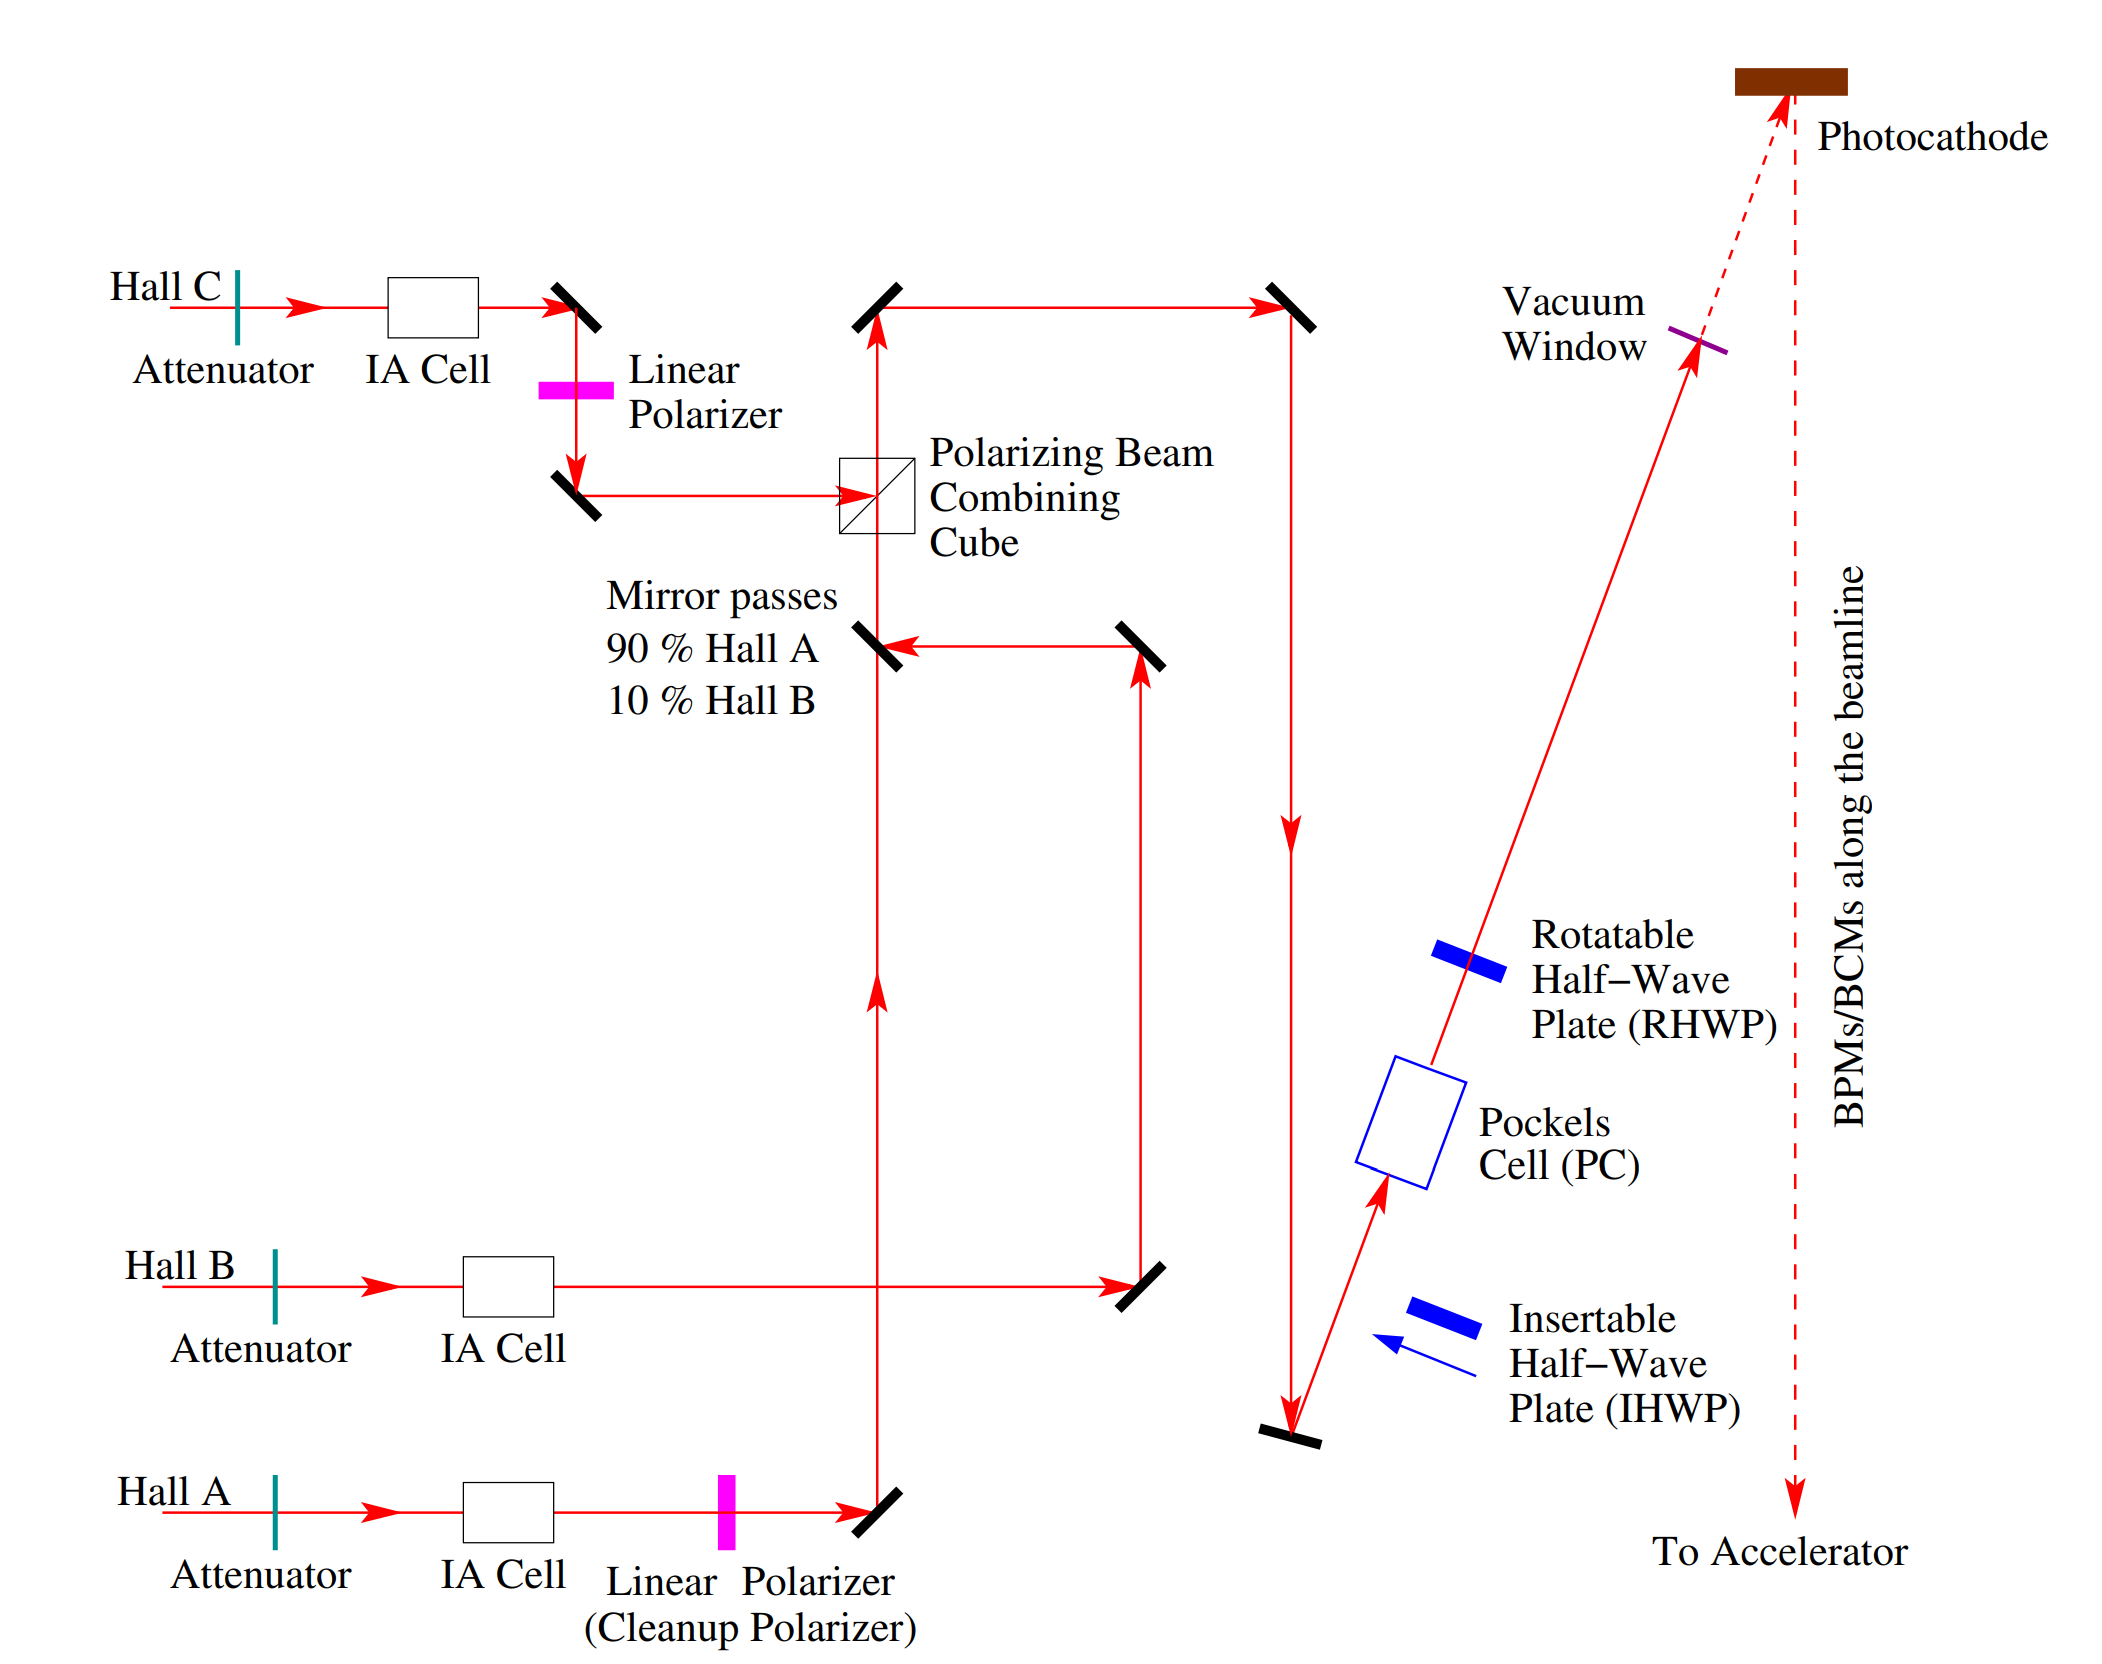
\includegraphics[width=\textwidth]{images/chap3/jlab_polarized_source.png}
    \caption{Schema of the Polarized Laser system in the injector. add REF}
    \label{fig:cebaf_polarize_laser_system}
\end{figure}
\subsection{Polarized Beam Source}

The polarization of the electron beam is quantified by the following equation:

\begin{equation}
p = \frac{N{\uparrow} - N{\downarrow}}{N{\uparrow} + N{\downarrow}}
\end{equation}

Here, $N$ represents the number of electrons in the conduction band of each corresponding spin state. 

The generation of polarized electrons in our source is underpinned by the photoemission process from negative-electron-affinity III-V semiconductor materials, notably Gallium Arsenide (GaAs). The electron spin polarization observed arises from the unique crystal symmetry of GaAs, which governs transitions from the fully occupied valence band to the normally vacant conduction band, akin to transitions from a state with total angular momentum j=3/2 to one with j=1/2. For bulk GaAs as showed in the plot [todo ADD THE energy plot], permits two transitions between the valence band and the conduction band. For every given excitation, three times as many electron spins are anti-parallel to the photon spin than parallel to it. as a result, in theory the maximum polarization can achieve is $50\%$. But in practice, the polarization is around $30-40\%$. 


Addressing this limitation, T. Maruyama and colleagues at the Stanford Linear Accelerator (SLAC) pioneered the use of strained GaAs to increase the polarization rate, \cite{PhysRevLett.66.2376}. This approach achieved an enhanced polarization rate of approximately $70\%$. The technique of strained GaAs involves the epitaxial growth of an InGaAs surface layer on GaAs. The resulting crystal-lattice mismatch between these two compounds introduces an axial strain. This strain effectively breaks the degeneracy of the $P_{3/2}$ valence band energy levels, thereby providing a mechanism to restrict optical excitation from the undesired valence-band spin state. This advancement represents a significant stride in the optimization of electron beam polarization. However, strained GaAs has its own challenges, notably a lower quantum efficiency (QE), which is typically on the order of $0.1\%$. Efforts to augment the QE, for instance, by increasing the thickness of the strained layer, tend to result in a concomitant decrease in polarization, presenting a trade-off that must be carefully managed in practical applications.

The modern photocathodes employ a superlattice structure, composed of numerous thin-layer pairs of lattice-mismatched materials. This design amalgamates the advantages of numerous thin strained layers to simultaneously achieve high polarization and high QE. The photocathode uses in Jefferson Lab achieves approximately $90\%$ polarization while maintaining a quantum efficiency of about $1\%$. \cite{PhysRevB.13.5484}, \cite{ADDERLEY2023167710}


[bulk GaAs figure]

[strain GaAs figure]

[super-lattice GaAs figure]

[add energy level figure]

\subsection{Helicity Control}
Helicity plays a pivotal role in the PRex/CRex experiments. For the minimization of systematic errors, it is imperative to quickly and consistently flip the helicity, or spin direction, of the electron beam. The Pockels Cell (PC) is instrumental in facilitating this helicity reversal. This device is indeed crucial for the PRex experiment as it enables rapid, precise control over the electron beam's helicity, a vital requirement for measuring neutron distribution.

The heart of the Pockels cell consists of two piezoelectric crystals made of Rubidium Titanyl Phosphate. When voltage is applied to these crystals, they can transform linearly polarized laser light into either left or right circularly polarized light. This polarization alteration directly affects the helicity of the electron beam. By modulating the voltage applied to the crystals, the beam's helicity can be swiftly adjusted. For the PRex-II experiment, the helicity flip rate was set at 240Hz.[REF pockels cell board paper] 

\section{Beam monitor}

Numerous beam monitors operate within CEBAF (Continuous Electron Beam Accelerator Facility) to ensure its functionality aligns with the experimental requirements. Among these monitors, the polarimeter, beam position monitor, and beam current monitor play significant roles in the success of the PRex/CRex experiments. This section provides a concise introduction to these vital monitoring systems, offering an insight into their operations and their importance in maintaining the integrity of the experiment.

\subsection{polarimeters}

\subsubsection{Mott Polarimeter}



\subsubsection{Compton Polarimeter}

The Compton polarimeter in Jefferson Lab's Continuous Electron Beam Accelerator Facility (CEBAF) Hall A is another essential instrument used to measure the polarization of the electron beam. Unlike the Møller polarimeter, which relies on electron-electron interactions, the Compton polarimeter operates based on the principle of Compton scattering.

Compton scattering involves the interaction between a beam of electrons and a photon, typically originating from a laser. The electrons scatter off the photons and experience a change in energy and direction depending on the incident photon's energy and the scattering angle. The change in energy of the scattered electrons (or alternatively, the scattered photons) is directly related to the polarization of the incident electron beam.


In the Compton polarimeter in Hall A, the beam is directed into the optical cavity by two dipole magnets. A high-powered, circularly polarized laser is strategically positioned inside the cavity to intersect the electron beam. This encounter leads to Compton scattering, thereby generating scattered photons and electrons. However, only a minute fraction of the electron beam interacts with the polarized photons. Post-scattering, the beam is deflected back to the beam line. The scattered electrons are detected using electron detectors, which comprise plates of synthetic diamonds developed through chemical vapor deposition. Compton-scattered photons are identified within an array of lead tungstate (PbWO4) crystals.

A unique advantage of the Compton polarimeter is its capacity to assess the beam's polarization without disrupting its operation. This feature facilitates uninterrupted, real-time monitoring of the beam's polarization during experiments. The disparity in count rates between the two helicity states serves as an indicator of the beam's polarization, thereby enhancing the accuracy and reliability of the measurements.


\begin{figure}[!htbp]
    \centering
    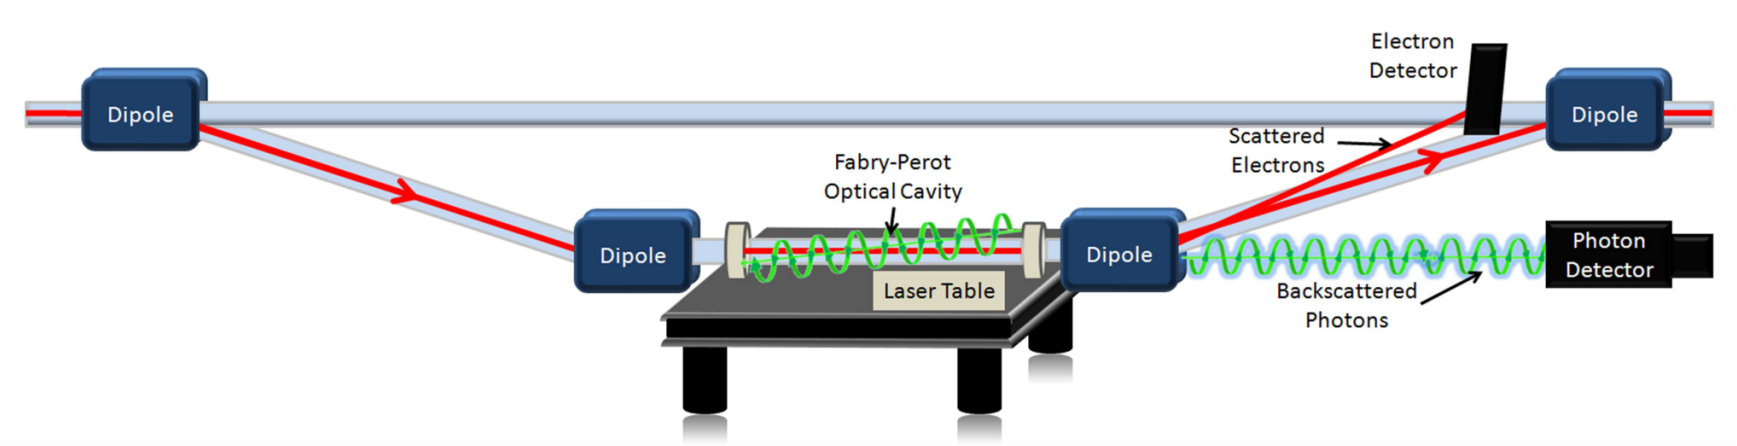
\includegraphics[width=\textwidth]{images/chap3/compton.png}
    \caption{Caption}
    \label{fig:enter-label}
\end{figure}


% \begin{equation}
%     A_{exp} = \frac{n^+-n^-}{n^++n^-} = P_{\gamma}P_e<A_{th}>
% \end{equation}

\subsubsection{Moller Polarimeter}

The Møller polarimeter operates by detecting the electrons scattered from a polarized target, leveraging the phenomenon known as Møller scattering. This type of electron-electron scattering happens when two electrons interact, and the outcome of this interaction is measured. Significantly, the probability of scattering is deeply influenced by the relative spin orientations of the interacting electrons. This property makes Møller scattering particularly beneficial for gauging beam polarization. Unlike the Compton polarimeter, however, the Møller polarimeter cannot operate simultaneously with the production run.

In the ultra-relativistic limit, the Møller asymmetry can be expressed as:

\begin{equation}
A_{exp} = P_{beam}P_{targ}<A_{zz}>
\end{equation}

In this equation, $<A_{zz}>$ represents the average analysis power over the captured cross-section, given by:

\begin{equation}
A_{zz} = \frac{\sin^2{\theta(7 + \cos^2{\theta})}}{(3 + \cos^2{\theta})^2}
\end{equation}

\begin{figure}[!htbp]
    \centering
    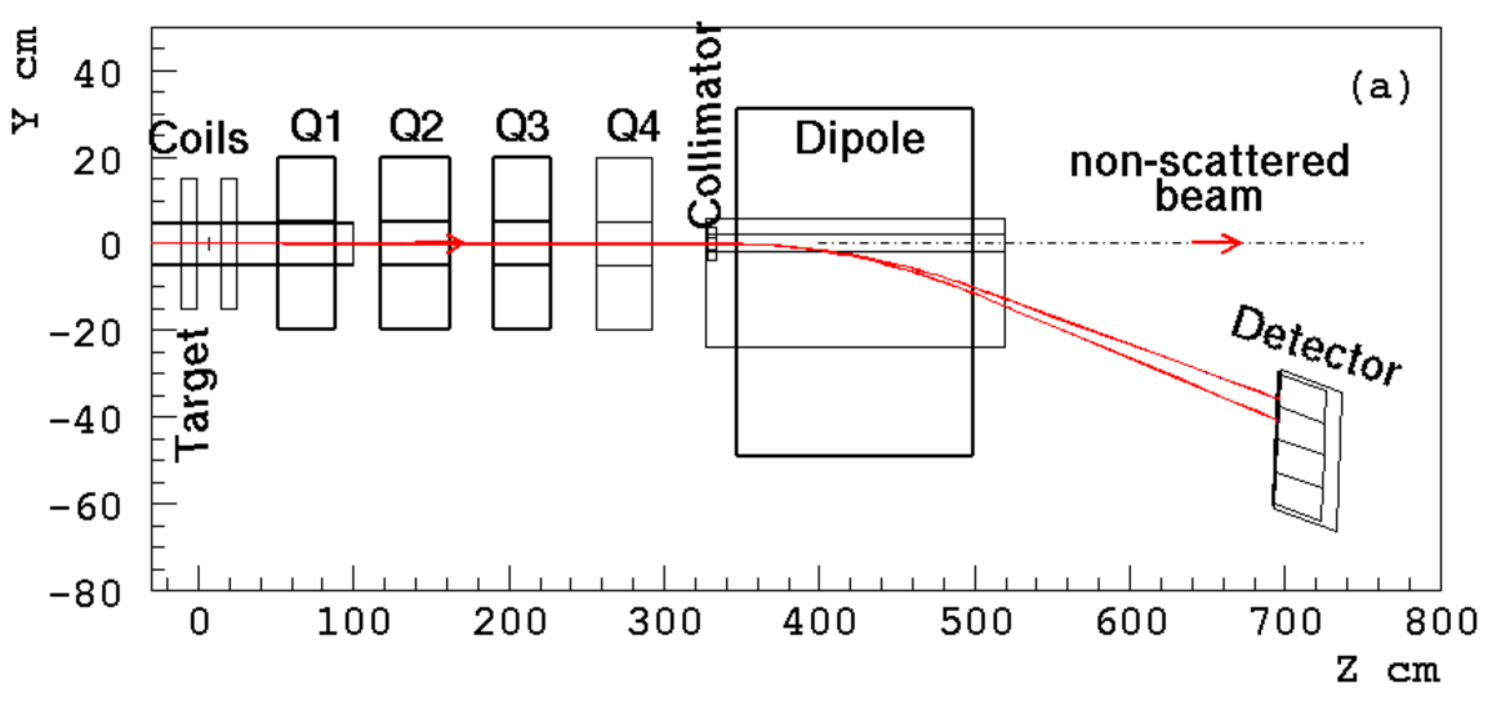
\includegraphics[width=\textwidth]{images/chap3/moller.png}
    \caption{moller, need to re-plot}
    \label{fig:enter-label}
\end{figure}

\subsection{Beam Position Monitor}

The beam position is a critical parameter for calculating the kinematics of electron scattering. Various Beam Position Monitors (BPMs) are installed throughout CEBAF to ensure the beam operates optimally. In the PRex-II/CRex experiment, two types of BPMs are mainly employed: one suited for high current beam position measurements, and a low current cavity monitor used when the beam current is low.

Each BPM features a four-wire antenna, placed diagonally along the beamline and denoted as $V_+$, $V_-$, $U_+$, and $U_-$. As the beam traverses the BPM, it induces a current in the antenna, the amplitude of which is proportional to the beam's position and intensity. Figure \ref{fig:cebaf_beam_position_monitor} illustrates the BPM's structure.

The position of the beam along the BPM's antenna-rotated coordinate system can be expressed as:

\begin{equation}
x' = c_x\frac{V_+ - V_-}{V_+ + V_-}
\end{equation}
\begin{equation}
y' = c_y\frac{U_+ - U_-}{U_+ + U_-}
\end{equation}

In these equations, $c_x$ and $c_y$ denote calibration constants. The hall coordinate system is rotated from the BPM's wire direction by $45^\circ$. With the rotation matrix, the position measured by the BPM in the hall coordinate system can be represented as:

\begin{equation}
x_{bpm} = x'\cos{\theta} - y'\sin{\theta}
\end{equation}
\begin{equation}
y_{bpm} = x'\sin{\theta} + y'\cos{\theta}
\end{equation}

Here, the rotation angle $\theta = 45^\circ$. Beam Position Monitor A (IPM1H03A, BPMA) is situated $7.524m$ upstream of the target, and Beam Position Monitor B(IPM1H03B, BPMB) is $1.286m$ upstream of the target.



\begin{itemize}
    \item cavity for low current measurement 
    \item harp for bpm collaboration
\end{itemize}

\subsection{Beam current monitor}

In the PRex-II and CRex experiments conducted at Jefferson Lab, the Beam Current Monitor (BCM) is used for the precise measurements of beam current and beam charge. Engineered for stability, minimal noise, and non-intrusive operation, the BCM is strategically situated about 25 meters upstream of the target.

At its core, the BCM features a Parametric Current Transformer (PCT) sensor, commonly known as an Unser monitor, and a pair of RF cavity monitors. The PCT toroid is designed to be responsive to the direct current (DC) component of the magnetic field, generated by the beam current as it encircles the beam pipe.

To mitigate the impact of parasitic currents, a ceramic gap interrupts the conductivity of the beam pipe within the toroid. Moreover, the system employs three magnetic shields—two comprised of iron and the innermost one of µ metal—to counteract offset drifts induced by fluctuating external magnetic fields.

The entire assembly is encased in a thermoregulated enclosure that further curtails PCT offset drifts. An electrical shield is implemented to prevent high frequencies in the beam spectrum from escaping the monitor via the ceramic gap. Additionally, materials with high absorption capacity are used to shield the sensor from RF noise, ensuring that the BCM consistently delivers accurate and reliable measurements.

\begin{figure}[!htbp]
    \centering
    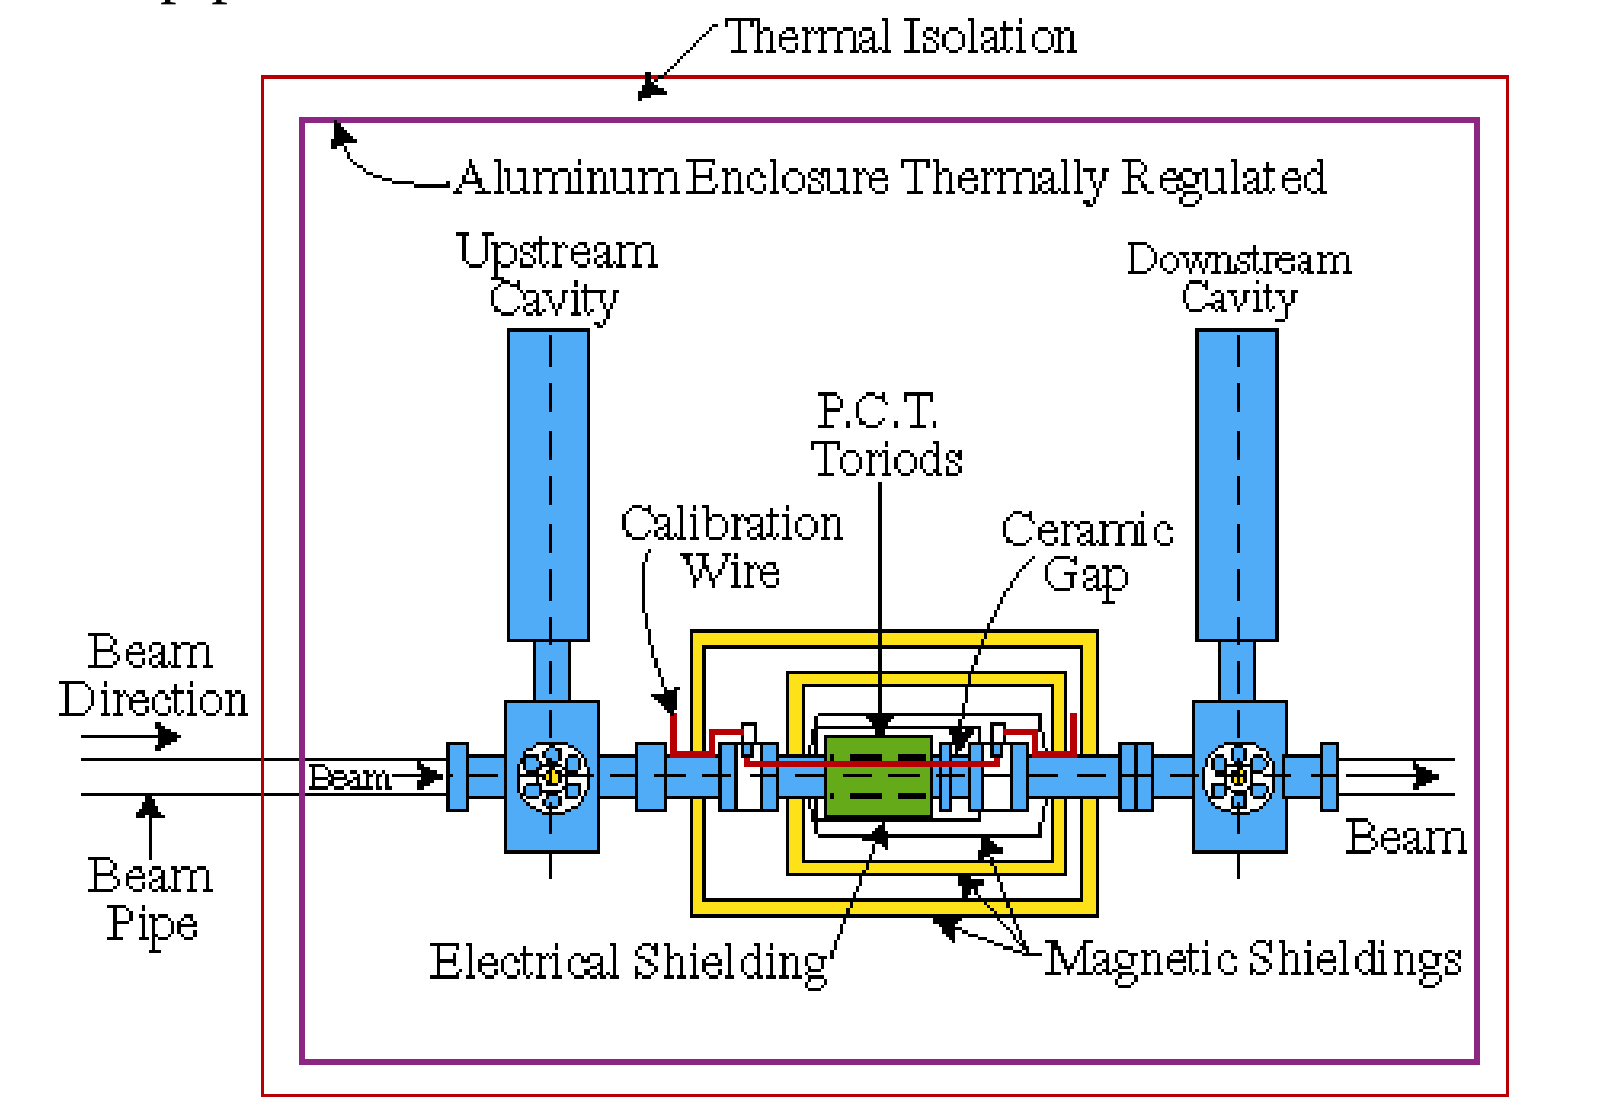
\includegraphics[width=\textwidth]{images/chap3/beam_current_monitor.png}
    \caption{Caption (SOURCE)}
    \label{fig:enter-label}
\end{figure}


\subsection{Raster}

Generally speaking, the beam size in Jefferson Lab's CEBAF is typically on the order of hundreds of micrometers (${\mu}m$) in diameter. This is a quite small size, which is why the beam can deposit a large amount of energy in a small area and why rastering is necessary when delicate or thin targets are used in experiments to avoid damage to the target.

In Hall A, the raster system includes two sets of air-core dipoles positioned upstream of the Compton polarimeter. Each set of dipoles is driven by an independent power supply, which allows for independent control of the horizontal and vertical dimensions of the rastered beam spot. In the PRex experiment, the rastered beam sport are set to $2cm \times 2 cm$ or $4cm \times 4cm$.

[....... to be added]

Para. to be added
\begin{itemize}
    \item spot++ [used to get the beam plot]
    \item rostered beam plot [find the slides]
    \item calibration of the raster on the beam position which will affect the momentum calibration HRS calibration [slides]
\end{itemize}

\subsection{Beam energy monitor, Tiefenhach measurement}

[..... to be added]

\section{Target System}

The experiments conducted in Jefferson Lab employ two separate target ladders, each hosting different types of targets for specific purposes. The production ladder is equipped with the main targets used for the experiments, while the optics ladder carries calibration targets.

Each target ladder is independently affixed to a motion system and can be controlled separately from the counting-house. As required, these targets can be positioned accurately along the central beamline during the experiment.

\begin{figure}[!htbp]
    \centering
    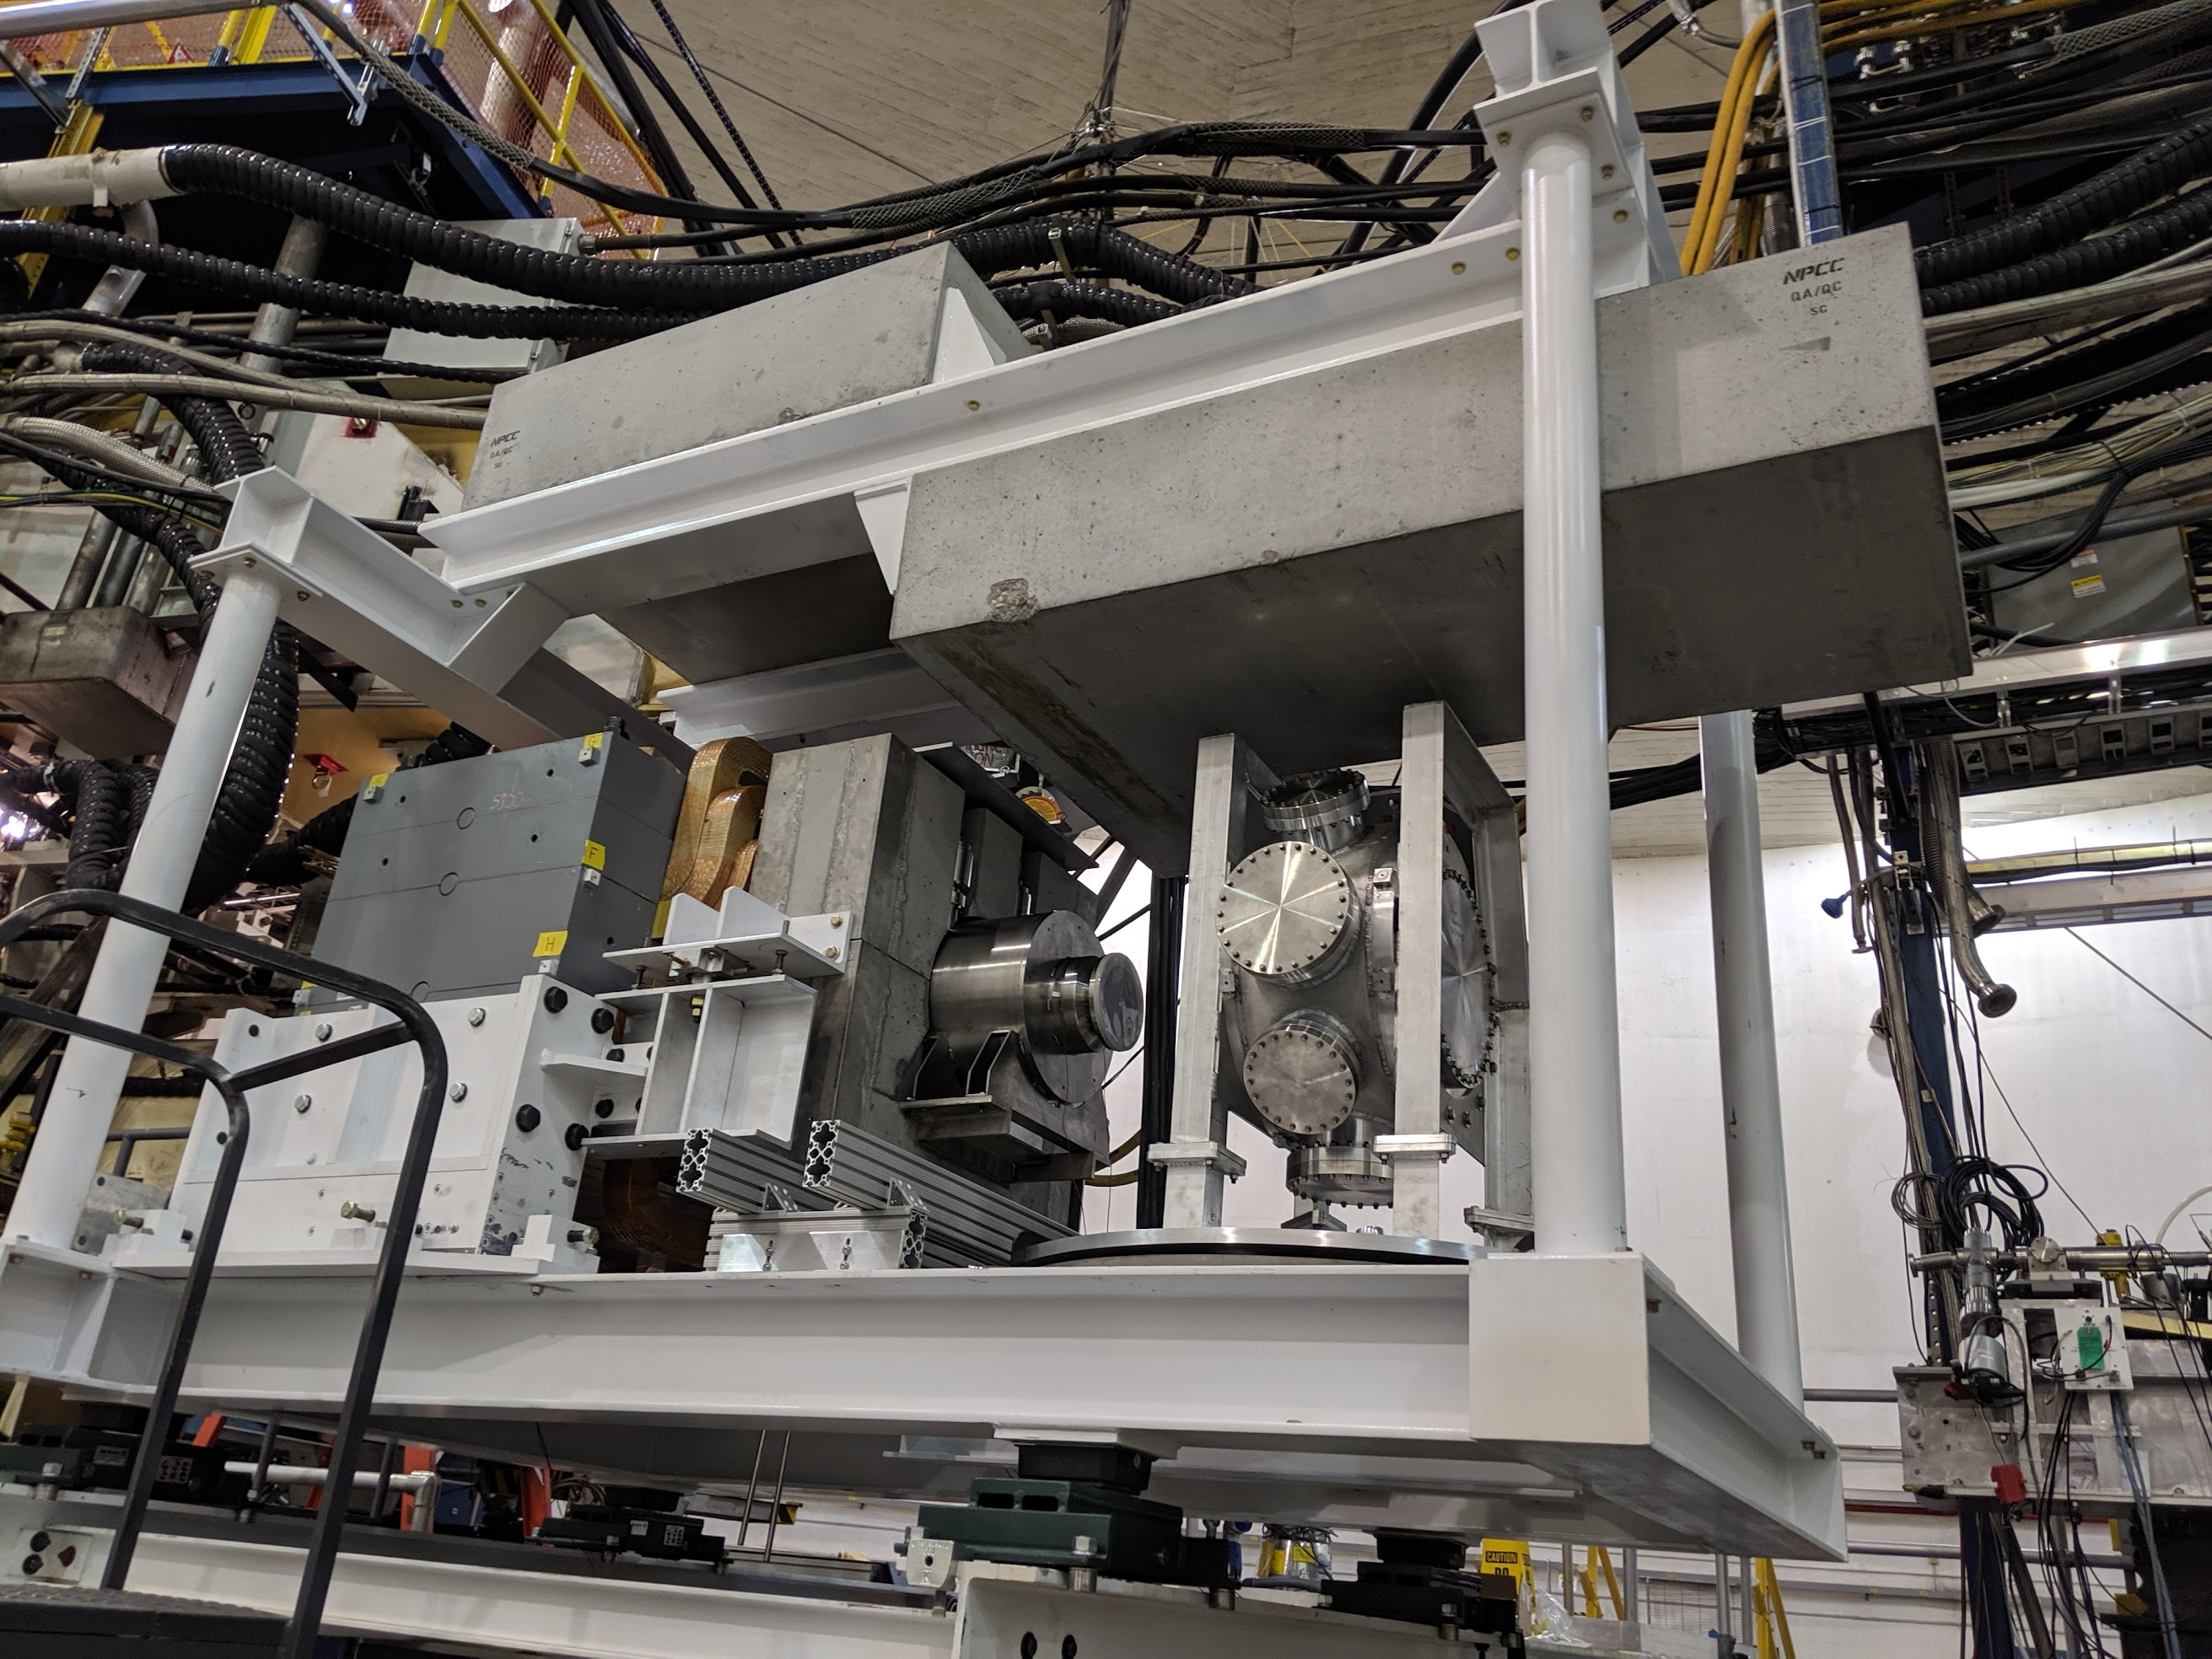
\includegraphics[width=\textwidth]{images/chap3/target_chamber.jpg}
    \caption{Target Chamber used in PRex-II/CRex experiment}
    \label{fig:target_chamber_photo}
\end{figure}

The production target ladder comprises ten 208Pb-D targets, a Carbon target at $1\%$ density, a Carbon hole target designed for alignment purposes, and a Ca48 target. To maintain their performance under high-intensity beam conditions, the targets on the production ladder are cooled with liquid helium at 15K. Of particular note for the PRex experiment are the 208Pb targets. These targets are approximately 0.5mm thick and sandwiched with diamond foils to enhance thermal conductivity, thereby helping to dissipate the power deposited by the beam.

The optics ladder, on the other hand, houses five targets used for High-Resolution Spectrometer (HRS) optics calibrations. These targets, cooled by water, include a natural Pb target, tungsten target, carbon foil target, carbon hole target, and a falling water target developed by INFN. Among them, the Carbon foil is employed for HRS optics calibration and the water target for pointing measurements. These measurements enable the accurate determination of the HRS angles. The detailed procedures related to these calibration processes will be thoroughly discussed in Chapter 5.

[... more]

\begin{itemize}
    \item Ca target
    \item carbon hole 
\end{itemize}




\section{High Resolution Spectrometer}

The High-Resolution Spectrometers (HRSs) in Hall A of Jefferson Lab are integral components designed specifically for precision measurements of scattering processes. Capable of high-precision particle detection, these instruments allow scientists to delve into the exploration of subatomic matter structures.

Hall A is equipped with two such HRSs, each capable of measuring momentum with an exceptional resolution of up to $0.01\%$. These spectrometers maintain a broad horizontal angular acceptance of ±28 milliradians (mr) and a vertical acceptance of ±60 mr. Strategically positioned on either side of the beamline, each spectrometer can rotate within a plane perpendicular to the beamline, accommodating angles between 12.5 to 150 degrees. This extensive angular range permits the spectrometers to capture scattered particles across a diverse spectrum of kinematic conditions.

In the context of the PRex and CRex experiments, both spectrometers are adjusted to detect scattered electrons at an angle of 5 degrees to maximizes the number of events collected during the experiment. To complement the minimum acceptance angle of the HRSs, an additional spectrometer magnet is incorporated to pre-bend the particles prior to their entry into the HRS.

Positioned within a shield house, the detector package is composed of a range of detectors, each designed for a specific role in measuring the attributes of scattered particles. The detectors are equipped to assess position, angle, and timing of incoming particles. This trio of information is pivotal in determining their momentum and classification, thus forming a comprehensive overview of the particle's properties.

[.... to be added, the HRS plot]

\subsection{Sieve slit Collimators}

The sieve slit collimators used in Jefferson Lab's Hall A High Resolution Spectrometers (HRS) are 0.2-inch-thick tungsten plates, precisely drilled with a regular pattern of holes. Each hole measures 0.05 inches in diameter, except for three larger holes that are 0.106 inches across, which are utilized to aid in the accurate location of the collimator holes.
\begin{figure}[!htbp]
    \centering
    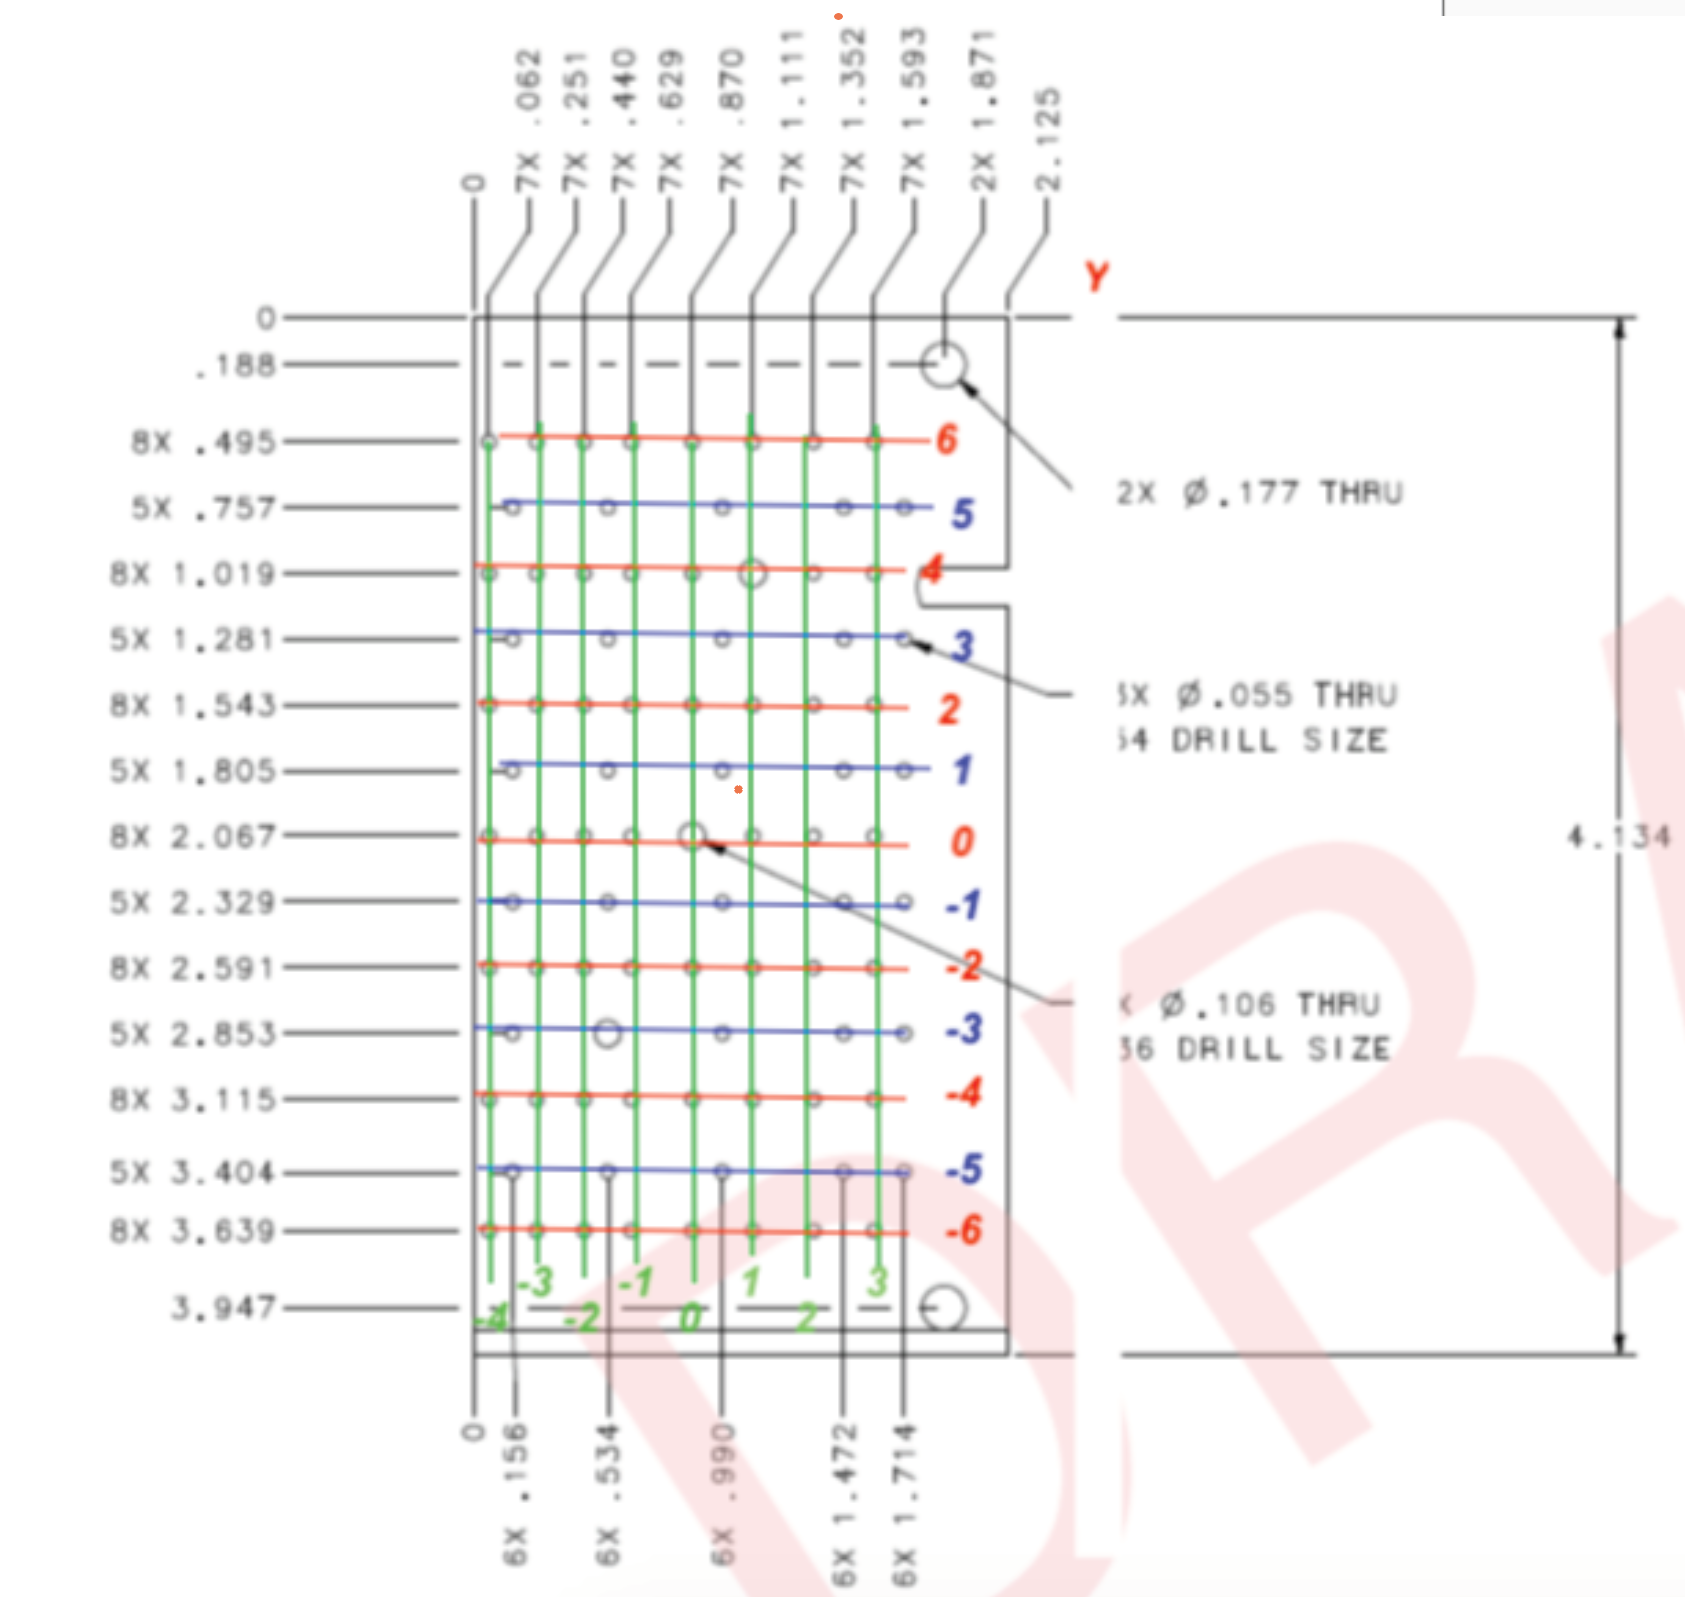
\includegraphics[width=0.5\textwidth]{images/chap3/sive_slit.png}
    \caption{Sieve slit used for PRex-II/CRex experiment [need to redraw]}
    \label{fig:enter-label}
\end{figure}
Each side of the HRS beamline is equipped with one sieve slit positioned at the beamline's entrance. The manufacture of these sieve slits involves high-precision Computer Numerical Control (CNC) machining and a thorough surveying process using laser technology, ensuring the utmost accuracy before the commencement of any experiment. The momentum of electrons passing through each sieve hole can be computed precisely, providing a robust reference for spectrometer calibration. Further details regarding the HRS calibration with sieve slits will be discussed in the subsequent chapter.

When the sieve slits are in place, only the electrons passing through these holes can reach the HRS. Each sieve slit is linked to a control unit, enabling manual placement or removal of the slit. During the production runs, the sieve is typically removed and only reinserted during optics runs. To ascertain the accuracy of this system, multiple optics runs were carried out throughout the experiment. 




\subsection{collimeter}

[... merge with the sieve slit?]


\subsection{Magnet Chain of the HRS}


\subsubsection{Septum Magnet}
\subsubsection{QQDQ magnet package}

\subsection{detector package}

\subsection{Vertical Drift Chamber}
\subsection{S0, S3 scintillator as trigger}
\subsection{Quartz, AT}
\subsection{GEM detector}

\section{GEM detector for the PRex/CRex experiment}
\begin{itemize}
    \item GEM foil
    \item GEM foil structure, microscope image
    \item GEM foil magnetic field simulation (Garfield simulation)
\end{itemize}


\begin{itemize}
    \item GEM detector structure
    \item AI window used de-polarized the window
    \item Window 
    \item 3 GEM layers
    \item Read out strips 
    \item backbone 
    \item back chamber used for balance the pressure, prevent the readout board bend
\end{itemize}


\begin{itemize}
    \item How GEM works
    \item Garfild simulation 
\end{itemize}

\section{GEM detector}
\subsection{HV}

\begin{itemize}
    \item High Voltage Regestor chain 
    \item HV models 
    \item High Voltage Scan
    \item the lowest voltage that meets the requirements
\end{itemize}

\subsection{LV}

\begin{itemize}
    \item The Low voltage power supply
    \item current consideration 
    \item images of the low voltage
    \item cooling 
\end{itemize}

\subsection{Gas Flow}

    \begin{itemize}
        \item The Gas flow system
        \item bubbler
        \item how to distribute to the chamber 
        \item gas flow in the chamber
    \end{itemize}

\subsection{DAQ system of the GEM detector}

\subsubsection{APV}
\begin{itemize}
    \item APV 25, charge sensitive pre-amplifier
    \item HDMI cable
    \item Noise Reduction technics (the fifth channel of the HDMI is not good)
\end{itemize}

\subsubsection{MPD}

\begin{itemize}
    \item analog to digital converter
    \item CPU 
    \item event rate limitations
\end{itemize}



\subsection{QUATZ / AT}
\subsection{trigger system}

